
\section{Formulation of the Core Radiation Scheme}

\subsection{Overview}

The purpose of the radiation code is to calculate radiative fluxes, 
from which heating rates and related 
quantities may be determined. In this radiation scheme these fluxes are 
determined by summing the 
results of a number of quasi-monochromatic calculations, each carried 
out using a two-stream 
approximation (in which the angular variation of the radiance field is
represented simply by an upward and a downward diffuse flux, together
with a direct solar flux in the shortwave region).
The algorithm can perhaps most clearly be explained by describing first 
the spectral 
integration in broad terms, then the treatment of the 
quasi-monochromatic calculations in an 
atmospheric column composed of homogeneous layers, working backwards to 
the original physical 
inputs, before passing on to a discussion of the treatment of 
overlapping gaseous absorption and the 
treatment of fractional cloudiness. \\

\noindent
Spectral data for the parametrizations used and the decomposition of 
each spectral region into bands 
are stored in a {\em spectral file}, generated by a pre-processing 
package (see section~\ref{sec:spec} for further discussion of spectral files).
It is important to note that parametrizations which require 
spectrally dependent data may be 
selected only if such data are present in the spectral file, and 
therefore that parametrizations must be 
selected with due consideration to the spectral data available. Once 
created, a spectral file may be used 
with any subsequent version of the radiation code.

\subsection{Spectral Integration}

In this section $F$ will denote any flux, whether direct, diffuse or 
net. The spectral region under 
consideration is divided into a number of spectral bands within which 
all quantities except the gaseous 
mass absorption coefficient are treated as independent of frequency. 
The total flux is then the sum 
over the partial fluxes, $F^{(b)}_{j}$, in each of the bands:
\beq
F=\sum_{j} F^{(b)}_{j}
\label{p2_eq1}
\eeq 
The flux in a band is calculated by dividing the band into a number of 
quasi-monochromatic regions 
in each of which the gaseous absorption coefficients for the active 
absorbing gases within the band 
have fixed values. A weight, $w_{k}$, is assigned to the  $k^{th}$ 
region, and the flux, taking the appropriate 
values of the gaseous absorption coefficients
into account, is calculated for this 
region. The flux in the band is then 
a weighted sum of these quasi-monochromatic fluxes, $F^{(qm)}_{k}$      
        
\beq
F^{(b)}_{j}=\sum_{k} w_{k} F^{(qm)}_{k}
\label{p2_eq2}
\eeq 
The number of quasi-monochromatic calculations and the weights are 
determined by the method 
adopted for treating overlapping gaseous absorption and the data in 
the spectral file.

\subsection{The Calculation of Monochromatic Fluxes}

To calculate monochromatic fluxes the atmosphere is divided into $N$ 
layers which are treated as homogeneous. The layers are numbered from 1 
to $N$, starting at the top. The boundaries of these layers, referred to 
as levels, are numbered from 0 to $N$, again starting at the top; so that 
the $i^{th}$ level marks the base of the  $i^{th}$ layer (see Fig.\ref{CMF1}). 
The layers match those adopted elsewhere in the model, with the interior 
boundaries corresponding to the $\rho$-levels $2,\ldots, N$, although inverted;
the first $\rho$-level is omitted on the physics grid. Increments to the 
heating rates are applied on $\theta$-levels.
\begin{figure}
\begin{center}
\includegraphics[width=8.0cm,angle=270]{layer.ps}
\caption{Vertical Resolution of Atmosphere}
\label{CMF1}
\end{center}
\end{figure}
\noindent
In order to minimize the execution time, it is convenient to choose the 
upward flux, $U$ , the total downward (diffuse plus direct) flux, $V$, 
and the direct solar flux, $Z$  , as the primary variables in the solar region 
(notice the non-standard choice of the total rather than the diffuse 
downward flux which allows a slight reduction of the operation count). In the 
infra-red it is convenient to use the upward and downward differential 
fluxes (the actual upward and downward fluxes less $\pi B$ ), which we here 
denote as $U$  and $V$  to achieve a unified description valid in both spectral 
regions. For applications where only heating rates or net fluxes 
are required, it is often convenient to work with the net flux $N=V-U$.
The fluxes in a column consisting of homogeneous layers are then determined 
from the equations:
\beqn
U_{i-1} & = & T_{i} U_{i}+ R_{i}V_{i-1}+S^{+}_{i} \nonumber \\
V_{i}   & = & T_{i} V_{i-1} + R_{i} U_{i}+S^{-}_{i} \\
Z_{i}   & = & T_{0i} Z_{i-1} \nonumber
\label{p2_eq3}
\eeqn
$T$  and $R$ are the diffuse transmission and reflection coefficients 
and $T_{0}$ is the direct transmission 
coefficient. The subscripts on fluxes refer to levels and those on  
$T$, $R$ , $T_{0}$ and $S$ refer to layers. 
At the top of the atmosphere there is no incident diffuse flux, so the 
boundary condition for solar 
radiation is $V_{0} =Z_{0}=\Phi_{0}/\chi_{0}$ where $\Phi_{0}$ is the 
solar irradiance in the band at the top of the 
atmosphere and $\chi_{0}$  is the secant of the solar zenith angle. In 
the infra-red, the boundary condition 
is $V_{0}=0$ . At the surface the appropriate boundary condition on the 
shortwave fluxes is
\beqn
U_{N} & = & (\alpha_{s}-\alpha_{d})Z_{N}+\alpha_{d} V_{N} \nonumber \\
      & = & \alpha_{s} Z_{N} +\alpha_{D}(V_{N}-Z_{N})
\label{p2_eq4}
\eeqn 
where $\alpha_{s}$  and $\alpha_{d}$  are the surface albedos for 
direct and diffuse radiation. In the infra-red
\beq
U_{N}=\alpha_{d} V_{N} + \epsilon_{*} \pi B_{*}
\label{p2_eq5}
\eeq 
where $\epsilon_{*}$ is the emissivity of the surface and $B_{*}$ is 
the corresponding Planckian function.\\

\noindent
The source terms, $S^{\pm}$, are related to the direct solar flux (scattering 
of the direct beam into diffuse radiation) or to variations in the Planckian source 
function across the layer, as appropriate to the spectral region. In the solar spectrum,
\beq
S_{i}^{+}=c_{1i}Z_{i-1} \ \  \textrm{and} \ \ S^{-}_{i}=c_{2i}Z_{i-1}
\label{p2_eq6}
\eeq
where the $c_{j}$ depend on the properties of the layer and
are considered below. In the infra-red
\beq
S_{i}^{+}=c_{1i}\Delta_{1i}+c_{2i} \Delta_{2i} \ \  \textrm{and} \ \ 
S^{-}_{i}=-c_{1i}\Delta_{1i}+c_{2i}\Delta_{2i}
\label{p2_eq7}
\eeq
where $\Delta_{1}$ and $\Delta_{2}$ are related to the first and second 
differences of the Planck function across the 
layer, and terms involving $\Delta_{2}$ are present only if the 
Planckian source function is assumed to vary quadratically 
across the layer. Explicitly,
\beqn
\Delta_{1i} & = & B_{i}-B_{i-1} \nonumber \\
\Delta_{1i} & = & 2(B_{i}+B_{i-1}-2B_{i}^{(m)})
\label{p2_eq8}
\eeqn
where $B$ denotes the Planckian function integrated across the band at 
the appropriate level in the 
atmosphere and $B^{(m)}_{i}$ denotes the Planckian  function at the 
middle of the  $i^{th}$ layer. $B$ is given 
by a polynomial:
\beq
B=\sum^{n}_{k=0} \beta_{k} ( \theta/\theta_{R})^{k} 
\label{p2_eq9}
\eeq
where the order of the polynomial, n, the coefficients $\beta_{k}$ and 
the reference temperature, $\theta_{R}$, are 
determined externally.\\

{\it Note: In stand-alone radiation codes, it is usual to take the
variation of the Planckian as linear across layer. In the Unified Model,
because of the way in which temperatures are interpolated to the
edges of layers and the weakness of non-radiative damping in the
stratosphere, this led to the build up of two-grid-length waves
on the timescale of about a month. The quadratic variation was introduced
to allow these to be damped in climate integrations.}


\subsection{The Calculation of Fluxes}

$T$, $T_{0}$, $R$ and the  $c_{j}$ are related to the optical 
properties of the layer. Since each layer may be 
considered independently, the subscript $i$ will be dropped  in this 
section. The fundamental single scattering properties 
of a layer are the optical depth, $\tau$, the albedo of single 
scattering, $\omega$, and the asymmetry $g$ . The 
precise way in which these determine the overall transmission and 
reflection coefficients depends on the actual 
two-stream approximation selected (there are several two-stream 
approximations: see, for example, \cite{Zdunkowski80ts}).
Here they determine two quantities $s$  and $d$ in the 
first instance. Usually the two-stream 
equations are expressed in terms of the diffuse fluxes, $F^{\pm}$ as
\beq
\frac{dF^{+}}{d\tau}=\alpha_{1}F^{+}-\alpha_{2}F^{-}-Q^{+}
\label{p2_eq10}
\eeq
\beq
\frac{dF^{-}}{d\tau}=\alpha_{2}F^{+}-\alpha_{1}F^{-}-Q^{-}
\label{p2_eq11}
\eeq
where $Q^{\pm}$ are source terms: In terms of the variables used here, 
$s=\alpha_{1}+\alpha_{2}$ and $d=\alpha_{1}-\alpha_{2}$.\\ 

\noindent
In the Eddington approximation,
\beqn
s & = & \frac{3}{2}(1-\omega g) \nonumber \\
d & = & 2 (1- \omega)
\label{p2_eq12}
\eeqn
Using the approximation given by \cite{Zdunkowski85}, which we 
denote as PIFM85,
\beqn
s & = & D-\frac{3}{2}\omega g \nonumber \\
d & = & D (1- \omega)
\label{p2_eq13}
\eeqn 
where $D$ is the diffusivity factor, which is taken as 2 by these 
authors, though 1.66 is more 
commonly used in the infra-red to agree with Elsasser's value. The 
original version of the 
approximation given by \cite{Zdunkowski80ts} is
 \beqn
s & = & 2-\frac{3}{2}\omega g - \frac{1}{2} \omega \nonumber \\
d & = & 2 (1- \omega)
\label{p2_eq14}
\eeqn
This approximation follows less naturally from the derivation, but 
agrees more closely with 
reference results in the solar region. Using discrete ordinates,
 \beqn
s & = & \sqrt{3}(1-\omega g) \nonumber \\
d & = & \sqrt{3}(1- \omega)
\label{p2_eq15}
\eeqn
Under the Hemispheric mean approximation,
 \beqn
s & = & 2(1-\omega g \nonumber) \\
d & = & 2(1- \omega)
\label{p2_eq16}
\eeqn
These quantities determine the diffuse transmission and reflection 
coefficients:
\beqn
\lambda & = & \sqrt{sd} \nonumber \\
p       & = & e^{-\lambda \tau} \nonumber \\
\Gamma  & = & \frac{s-\lambda}{s+\lambda} \nonumber \\
T       & = & \frac{p(1-\Gamma^{2})}{1-p^{2} \Gamma^{2}} \nonumber \\
R       & = & \frac{\Gamma(1-p^{2})}{1-p^{2}\Gamma^{2}} = \Gamma (1-pT)
\label{p2_eq17}
\eeqn
In the infra-red,
\beqn
c_1 & = & \frac{1-T+R}{s \tau} \nonumber \\
c_2 & = & -\frac{1}{s \tau}\bigg[1+R+T-2 \frac{1-T-R}{\tau d}\bigg]
\label{p2_eq18}
\eeqn
It will be noticed that these expressions become indeterminate in the 
limit $\tau \rightarrow 0$ . This  
indeterminacy is removed by adding a small tolerance (the square root 
of the precision of the machine) 
to the terms $s \tau$, $d \tau$, $1-T+R$, and $1+R+T$. However, when 
$\tau$ is very small we prefer to use 
the asymptotic form for the second term within square brackets in 
$c_{2}$  {\it viz.}:
\beq
2\frac{1-T-R}{\tau d} \approx 2- \tau d
\label{p2_eq19}
\eeq
To define the $c_{j}$ in the solar region we introduce the quantity 
$\xi_{0}$, where
\beq
\xi_{0}=\frac{3g}{2 \chi_{0}}
\label{p2_eq20}
\eeq
for all the above two-stream approximations, except the discrete 
ordinate approximation, for 
which
\beq
\xi_{0}=\frac{\sqrt{3}g}{\chi_{0}}
\label{p2_eq21}
\eeq
In this spectral region we now define
\beq
f=\omega \frac{\chi_{0}}{2}
\label{p2_eq22}
\eeq
\beqn
\nu_{+} & = & f(s-\chi_{0}-\xi_{0}(d-\chi_{0})) \nonumber \\
\nu_{-} & = & f(s+\chi_{0}+\xi_{0}(d+\chi_{0})) 
\label{p2_eq23}
\eeqn
Then,
\beqn 
c_{1} & = & (\nu_{+}-R(1+\nu_{-}))-\nu_{+}T T_{0} \nonumber \\
c_{2} & = & T_{0}(1+\nu_{-} -R \nu_{+})-(1+\nu_{-}) T
\label{p2_eq24}
\eeqn

\subsection{Rescaling of the Single Scattering Properties}

The rather crude representation of the angular variation of the 
radiance in the two-stream 
equations causes unacceptable inaccuracies in the representation of 
scattering. However, these 
errors can be substantially reduced by the $\delta$-rescaling transformation 
(\cite{Joseph76}) which allows 
for the strong forward scattering exhibited by most atmospheric 
scatterers. A forward scattering 
fraction, $f$, is defined, using the standard prescription $f=g^{2}$  , 
and the single scattering properties are 
rescaled using the transformation
\beqn
\tau & \rightarrow & \tau(1- \omega f) \nonumber \\
\omega & \rightarrow & \omega(1-f)/(1- \omega f) \nonumber \\
g & \rightarrow & (g-f)/(1-f)
\label{p2_eq25}
\eeqn

\subsection{The Calculation of the Single Scattering Properties}

The single scattering properties most easily related to the 
physical sources are the mass extinction and 
scattering coefficients, $k^{(e)}$ and $k^{(s)}$, and the asymmetry $g$. 
When a number of optical processes 
are active in a region the contributions from each of them are combined 
in accordance with the 
formulae:
\beqn
k^{(e)} & = & \sum_{j} k_{j}^{(e)}, \nonumber \\
k^{(s)} & = & \sum_{j} k_{j}^{(s)}, \nonumber \\
g       & = &  \sum_{j} k_{j}^{(s)} g_{j}/ \sum_{j} k_{j}^{(s)} 
\nonumber \\
f       & = &  \sum_{j} k_{j}^{(s)} f_{j}/ \sum_{j} k_{j}^{(s)} 
\label{p2_eq26}
\eeqn
where, for each process, indexed by $j$, $f_{j}=g_{j}^{2}$. The optical 
depth and single scattering albedo are then 
determined from the formulae:
\beqn
\tau &= &k^{(e)} \Delta m \nonumber \\
\omega &=& \frac{k^{(s)}}{k^{(e)}}
\label{p2_eq27}
\eeqn
where $\Delta m$ is the column mass in the layer.

\subsection{The Representation of Single 
Scattering Properties for Individual Processes}

\subsubsection{Gaseous Absorption}

If there are $M$ active absorbing gases, $j=1,\dots, M$   in a band, each 
will enter a single quasi-monochromatic calculation with mass extinction
coefficients appropriate for the conditions of temperature and pressure
at each layer of the atmosphere.
The total contribution to the mass extinction coefficient is then
\beq
k^{(e,g)}=\sum^{M}_{j}K^{(g)}_{j} q_{j} f_{j}(p,\theta)
\label{p2_eq28}
\eeq
where $K^{(g)}_{j}$ is a mass extinction coefficient at reference pressure
and temperature, $q_{j}$ is the mixing ratio of the $j^{th}$ gas and $f_{j}$ is 
the  scaling function, which allows for variations in the
pressure, $p$, and the temperature, $\theta$. The scaled extinction
coefficients may be interpolated directly from a look-up table in the
spectral file which is now the preferred method. Alternatively, scaling
functions may be used of which two forms for $f$ are allowed within the code:
\beq
f=\bigg(\frac{p+\Delta}{p_{0}+\Delta}\bigg)^{\alpha} 
\bigg(\frac{\theta}{\theta_{0}}\bigg)^{\beta}
\label{p2_eq29}
\eeq
\beq
f=\bigg(\frac{p+\Delta}{p_{0}+\Delta}\bigg)^{\alpha} 
\bigg[1+A\bigg(\frac{\theta-\theta_{0}}{\theta_{0}}\bigg)
+B\bigg(\frac{\theta-\theta_{0}}{\theta_{0}}\bigg) ^{2}\bigg]
\label{p2_eq30}
\eeq
The second form is generally preferred as being more flexible and 
cheaper  to compute. The free parameters $\alpha$,
$\beta$, $\Delta$, $A$ and $B$ are determined by fitting to gaseous 
transmission data and are chosen such  that if 
they are given values of 0 then $f=1$. $p_{0}$  and $\theta_{0}$  are the 
reference pressure and temperature. $\Delta$  
represents the effects of Doppler broadening. A different scaling 
function may be used for each $k$-term, or one 
value may be used across the band; the latter is faster and originally
was commonly used, but we now tend to use separate scaling for each
term since this more accurate. 
All these choices are determined 
from the data in the spectral file.

\subsubsection{Self-broadening of gases}

If the mixing ratio of a gaseous absorber is close to unity,
pressure broadening due to collisions between molecules of the same
species will become important. The pressure-broadened width of a line
will depend on the volume mixing ratio of the gas, which is in the code
termed the gas fraction, and can be derived from the mass mixing ratios.

If dry mixing ratios are provided to the radiation code, then the gas
fraction of species $i$ is given by
\begin{equation}
\frac{n_i}{n_\text{tot}}
=\frac{n_i}{n_\text{tot, dry} + n_\text{H$_2$O}}
=\frac{\frac{n_i}{n_\text{tot, dry}}}
{1 + \frac{n_\text{H$_2$O}}{n_\text{tot, dry}}}
=\frac{\zeta_i \frac{m_\text{air, dry}}{m_i}}{1 + \zeta_\text{H$_2$O}
\frac{m_\text{air, dry}}{m_\text{H$_2$O}}},
\end{equation}
%
where $n_i$ is the number density of species $i$, $n_\text{tot}$ and
$n_\text{tot, dry}$ are the total air and dry air number density,
respectively, $\zeta_i$ is the mass mixing ratio
of species $i$, respectively, $m_i$ is the molar weight of species $i$
and $m_\text{air, dry}$ is the mean molar weight of dry air.

If mixing ratios include water vapour in the total density, then the
gas fraction is given by
\begin{equation}
\frac{n_i}{n_\text{tot}} =
\zeta_i \frac{m_\text{air, wet}}{m_i},
\end{equation}
%
where $m_\text{air, wet}$ is the mean molar weight of wet air. It is
given by
\begin{equation}
m_\text{air, wet}
=\frac{n_\text{tot, dry}}{n_\text{tot}} m_\text{air, dry}
+\frac{n_\text{H$_2$O}}{n_\text{tot}} m_\text{H$_2$O}
=\frac{m_\text{air, dry}}{1
+\left( \frac{m_\text{air, dry}}{m_\text{H$_2$O}} - 1 \right)
\zeta_\text{H$_2$O}} .
\end{equation}

\subsubsection{Continuum Absorption}

Theoretical models of gaseous absorption agree well with observations
at frequencies close to the centres of lines, but there remain some
discrepancies far from the centres which are represented by a smoothly 
varying {\em continuum} in radiation codes. Continua are not significant
for all gases and 
two continua are normally included in radiative calculations: the self 
and  foreign-broadened 
continua of water vapour. Their contribution to the mass extinction 
coefficient is
\beq
k^{(e,c)}=K^{(c)}_{f}q_{w}f_{f} n_{bf}+K^{(c)}_{s}q_{w}f_{s}n_{bs}
\label{p2_eq31}
\eeq 
where $q_{w}$ is the mixing ratio of water vapour, $f$ is the scaling 
function and $n_{b}$ is 
the molar density of the appropriate broadening species; the subscripts 
$f$  and $s$  stand for 
the foreign and self-broadened continua respectively. The coefficients 
$K^{(c)}_{f}$ and $K^{(c)}_{s}$  
are determined externally by fitting and the coefficients are read from 
the spectral file. For the 
self-broadened continuum, the broadening species is water vapour, and 
for the foreign-broadened continuum 
it comprises all other species except water vapour. The same functional 
forms for the scaling function that were 
used in the treatment of gaseous absorption are employed here. In the 
Unified Model it is often 
convenient to combine the line data and the foreign continuum data, 
making use of the fact that in practice
$n_{bf}$  is almost exactly a function of the pressure and the 
temperature. $k$-terms are then determined for the combined transmission:
this is discussed further in section~\ref{sec:spec}.

There are a number of models for the continuum. The one used here is
originally based on the CKD model of \cite{Clough89}, which has been
developed as new observations to constrain it become available. The
updating of this model is an issue in the generation of spectral files,
rather than in the radiation code itself.

A more general continuum absorption parametrisation, which also
supports collision-induced absorption (CIA), is also available. Continuum
$k$-terms are derived in the same way as gaseous absorption $k$-terms. These
are tabulated as a function temperature only in units of absorption per mass
density of each of the two continuum gases [m$^5$/kg$^2$]. Overlapping
absorption between different continua, and continua and gaseous absorption is
treated as overlapping gaseous absorption, however, a continuum absorption
spectrum can also be assumed to be perfectly correlated to that of a
particular gas. The latter assumption is generally more accurate for the
water vapour continua than random overlap. The overlap treatment for a
particular continuum is specified in the spectral file, and defaults to
that selected for gases.

\subsubsection{Absorption and Scattering by Aerosols}

The radiation code contains provision for treating aerosols. This 
section is concerned only with
the description of the radiative treatment of aerosols within the code. 
The specification of mixing 
ratios and aerosol models is described in the UM documentation.\\

\noindent
For each species of aerosol in each spectral band the contributions to 
the total and scattering 
extinctions are simply set proportional to the mass mixing ratio of the 
aerosol: the constants of 
proportionality and the asymmetry are determined externally and read 
from the spectral file. There 
is no allowance for variations in the shape of the size distribution
within the model. 
Hence,
\beqn
k^{(e,a)} & = & \sum_{j} K_{j}^{(e,a)} q_{j}, \nonumber \\
k^{(s,a)} & = & \sum_{j} K_{j}^{(s,a)} q_{j}, \nonumber \\
g^{(a)}   & = &  \sum_{j} K_{j}^{(s,a)} q_{j} g_{j}/ k^{(s,a)}
\label{p2_eq32}
\eeqn
where the sum is taken over all the species of aerosols present and the 
mixing ratios are denoted 
by $q_{j}$. Parametrizations of the influence of 
humidity on the optical properties 
hygroscopic aerosols are included by the use of a look-up table in
the humidity. This look-up table is read from the spectral file.

\subsubsection{Rayleigh Scattering}

Rayleigh scattering is represented by adding to the scattering and 
total extinctions a constant value 
for each spectral band, again determined externally and read from the 
spectral file. The 
asymmetry for Rayleigh scattering is 0.

\subsubsection{Absorption and Scattering by Water Droplets}

The single scattering properties in a cloud clearly depend on the
mass mixing ratio of water $L$ and of ice $I$, but they also depend
critically on the size of cloud particles, which can vary considerably.
It is therefore important that the radiation code should include a
treatment of the effect of particle size. A full scattering calculation 
for the whole size distribution is not possible, so a parametrization
in terms of a radiatively appropriate size is used. For water droplets
the effective radius is always used.

The properties of water droplets, then,  are determined from the mass mixing 
ratio of liquid water, $L$, 
and the effective radius of the droplets, $r_{e}$, using an appropriate 
parametrization, which may take various different forms. 
With the parametrization of 
\cite{Slingo82},
\beqn
k^{(e)} & = & L(a+b/r_{e}) \nonumber \\
k^{(s)} & = & k^{(e)}(1-c-d r_{e})  \nonumber \\
g       & = & e+fr_{e}
\label{p2_eq33}
\eeqn 
where the constants $a, \dots, f$ are determined externally and vary
with spectral band. An 
alternative is the parametrization of 
Ackerman and Stephens (\cite{Ackerman87}) as extended by
\cite{Hu93}:
\beqn
k^{(e)} & = & L(a_1 r_{e}^{b_2}+c_1) \nonumber \\
k^{(s)} & = & k^{(e)}(1-a_2 r_{e}^{b_2}-c_2 ) \nonumber \\
g       & = & a_3 r_{e}^{b_3}+c_3
\label{p2_eq34}
\eeqn 
Again, the $a_{j}$, $b_{j}$  and the $c_{j}$  are determined externally 
by fitting and are read from the spectral file.
{\it Note: Whilst this parametrization is more flexible than that of
\cite{Slingo82}, we have not used in practice because of the
expense of calculating exponentials}.

For fitting over a wide range of sizes, a parametrization with more
free terms is required. A scheme based on the use of Pad\'e approximants
has therefore been introduced
\beqn
k^{(e)} & = & L { {p_1 + p_2 r_e + p_3 r_e^2} \over 
                  { 1 + p_4 r_e + p_5 r_e^2 + p_6 r_e^3} } \nonumber \\
k^{(s)} & = & k^{(e)} \left(1 -{ {p_7 + p_8 r_e + p_9 r_e^2} \over 
                  { 1 + p_{10} r_e + p_{11} r_e^2 } }\right) \nonumber \\
g       & = & {p_{12} + p_{13} r_e + p_{14} r_e^2} \over
                  { 1 + p_{15} r_e + p_{16} r_e^2 }
\label{p2_xx0}
\eeqn
Section~\ref{sec:spec} should be consulted for information on the fits
available in the spectral files.

\subsubsection{Absorption and Scattering by Ice Crystals}

Conceptually, the treatment of scattering by ice crystals is similar
to that used for water vapour, but there are complexities because of
the irregular shape of crystals. From the point of view of parametrizations,
it is important to be aware that a number of different measures of
crystal size are in use, and that different schemes are based on
different measures.
Thus, if the prediction of crystal size in the model is
altered, it is important to be sure what is used by the radiation
scheme.

The simplest scheme is to proceed by analogy with water clouds and
to use a parametrization similar in form to that of \cite{Slingo82}:
 \beqn
k^{(e)} & = & I(a+b/r_{e}) \nonumber \\
k^{(s)} & = & k^{(e)}(1-c-d r_{e})  \nonumber \\
g       & = & e+fr_{e}
\label{p2_eq35}
\eeqn 
where the constants $a,\dots,f$ are determined externally. We stress that 
this scheme is based on the use of $r_e$ to measure the size. Schemes of
this form were used in HadAM3.

A more elaborate and better scheme is based on the modified anomalous
diffraction approximation (\cite{Mitchell96rp}). In this scheme,
the size of crystals is specified using the mean maximum dimension of
the large mode, $\bar D_l$. $\bar D_l$ is not a natural measure of
size for radiative purposes, but in this scheme, the underlying
(bimodal) size distribution is characterized by a single free
parameter, for which $\bar D_l$ is an acceptable choice, since once
a particle shape is specified there is a bijective relationship between
$\bar D_l$ and $r_e$. $\bar D_l$ varies by over two orders of magnitude
in this scheme so a fairly elaborate fit is required. This has been done
in two ways. The original form consists of two quartic polynomials for
the small and large ranges of $\bar D_l$. We define $x=\log(\bar D_l /D_T)$
where $D_T$ is a transitional dimension, supplied with the parametrization. 
Then,
\beqn
k^{(e)} & = & I \exp \left (\sum_{j=0}^4 a_j^\pm x^j \right ) \nonumber \\
k^{(s)} & = & k^{(e)} \left (1-\sum_{j=0}^4 b_j^\pm x^j \right )  \nonumber \\
g       & = & \sum_{j=0}^4 c_j^\pm x^j
\label{p2_xx2}
\eeqn 
where $a_j^\pm$,  $b_j^\pm$ and $c_j^\pm$ are constants supplied with the
parametrization, the sign being chosen according as $x>0$ or $x<0$.

For the published comparison of the scheme with runs in CCM3 
(\cite{Kristjansson99}, \cite{Kristjansson00}) a slightly
different form based on tenth order polynomials in $\bar D_l$ was developed.
This scheme represents the same data and, numerical differences in
the fit aside, is identical to the matched quartic scheme. 

Different crystal shapes may be represented within this same methodology,
but data in the standard spectral files are based on planar polycrystals
as these are the single most representative shape available amongst those
to which Mitchell's scheme is applicable.

A number of parametrizations for the single scattering properties of 
ice crystals have been suggested by various authors, based on an effective
dimension, $D_e$ or $D_{ge}$, as the measure of size. These are proportional
to the ratio of volume to projected area, and, for a sphere, $D_e$ is 
equal to the diameter. A parametrization in $D_e$ based on both the SW and
LW parametrizations of \cite{Fu96} and \cite{Fu98} has been
developed:
\beqn
k^{(e)} & = & I \sum_{j=0}^2 a_j / D_e^j  \nonumber \\
k^{(s)} & = & k^{(e)} \left (1-\sum_{j=0}^3 b_j D_e^j \right )  \nonumber \\
g       & = & \sum_{j=0}^3 c_j D_e^j
\label{p2_xx3}
\eeqn 
To some extent, using $D_e$ obviates the need to know the crystal shape
(but see \cite{Mitchell02}); however, one may need to know the crystal 
shape to determine $D_e$.

The specification of crystal size is an important issue in these 
parametrizations. The size is supplied as an input field to the radiation 
code. In the Unified Model it is generally parametrized as a function of
temperature only.

\cite{Baran09} and \cite{Baran12} argue that ice crystal optical properties 
should be linked directly to GCM prognostic variables rather than indirect 
diagnosed quantities such as $D_e$. Three such parametrizations are available; 
the first relates the optical properties to ice water content and temperature 
as described by \cite{Baran13}. The second depends on ice water content only as
described by \cite{Baran14}. The third is based on the same ensemble of ice
crystals used by \cite{Baran14}, but reintroduces a temperature dependence.

The spectral file may contain data for a number of types of ice crystal,
and the types used may be selected at runtime. For a given type,
the form of parametrization is determined by the spectral file. Further
discussion of types in particular files is given in section~\ref{sec:spec}. 


\subsection{The Treatment of Overlapping Gaseous Absorption}

If several gases absorb in a spectral band which does not cover too 
large a range of frequencies, 
their spectral lines may be taken to overlap randomly. In representing 
this absorption using $k$-terms 
it is necessary to consider the overlap of each $k$-term for one gas 
with each $k$-term for every 
other gas active in the band. This full treatment of random overlap is 
available within the code, 
but it is computationally expensive, and computationally faster 
approximations to it are provided.\\

\noindent
Equivalent extinction is an extension of the method of FESFT 
(\cite{Ritter92}) in which the effects of 
minor gases are represented 
by a single absorption coefficient within the band, but that 
coefficient is determined for the local 
atmospheric conditions by a  subsidiary calculation. In the infra-red 
region, supposing a minor gas 
to have $k$-terms $K_{r}$, $r=1, \dots,n$ the net flux, $N_{r}$  , 
including just absorption by 
the $r^{th}$ $k$-term of the gas (and any non-cloudy  grey 
absorption) is calculated. The equivalent 
extinction is then defined as
\beq
\bar{K}=\sum_{r} w_{r}K_{r}N_{r}/\sum_{r}w_{r}N_{r}
\label{p2_eq37}
\eeq
where the $w_{r}$ are the corresponding weights. A practical point 
concerning the numerical 
implementation of this approximation is that fluxes are calculated on 
levels, whereas the extinction 
coefficient must be a representative value in a layer. The equivalent 
extinction is therefore 
calculated using the mean net flux in the layer, which is taken as a 
simple average of the values 
at the boundaries. This is described more fully in \cite{Edwards96ek}.

\noindent
Two further variations of this method are available: the modulus
(absolute value) of the layer incident fluxes may be used in place of the
net fluxes in equation \ref{p2_eq37}. This should lead to increased
accuracy around temperature inversions where the net flux may change sign.
Where each $k$-term has different scaling characteristics a correction to
the method is also required so that the scaled values are used before
the meaning is done (this method also uses the modulus of the incident
fluxes to weight the $k$-terms in the LW).

\noindent
In the solar region it is less easy to define an equivalent extinction, 
since the character of 
downwelling radiation may be quite different from that of upwelling 
radiation, and the scheme 
adopted is provisional. For each minor gas the direct transmission 
through any atmospheric layer 
may be calculated and these transmissions are multiplicative, so the 
direct flux may be  calculated 
precisely and efficiently at all atmospheric levels. The calculation
of diffuse fluxes is less straightforward, but also much less critical,
given the particular spectral characteristics of the SW overlaps.
It is assumed that 
the absorption by the minor gas falls into weak and strong parts, so 
that radiation which is 
scattered into the diffuse beam will be effectively denuded in parts of 
the band where absorption 
is strong. If the remaining absorption is weak it may be treated as 
grey. The equivalent extinction 
for diffuse radiation is therefore taken to have a uniform value
\beq
\bar{K}=\sum_{r} w_{r}K_{r}Z_{*r}/\sum_{r}w_{r}Z_{*r}
\label{p2_eq38}
\eeq
where $Z_{*r}$ is the direct flux at the surface for the $r$th $k$-term. 
One further approximation is 
necessary to fit in with the calculation of cloudy transmission and 
reflection coefficients: in the 
calculation of source terms across a cloudy layer the direct flux is 
taken to vary from its true value 
at the top of the layer with the effect of minor gases being 
represented by the direct transmission 
calculated using the equivalent extinction.\\

\subsection{The Treatment of Clouds}

Two schemes are available for the treatment of cloud. In the original scheme,
a fairly general prescription is adopted where fluxes are solved for a single
column with fraction cloud cover.
Within any atmospheric layer, 
$i$, a fractional cloud cover, $W_{i}$, may be specified. This cloud is 
divided into $N_{T}$ {\em types}, each 
constituting a fraction, $\phi_{j}$ , of the total amount of cloud. 
Each of these sub-clouds is made up of 
mixtures of various {\em components}. The rule which determines how the 
components are partitioned 
between the types of cloud is termed a {\em representation}. For use in the 
Unified Model three 
representations are provided, depending on the treatment of ice and 
water clouds. Clouds consist 
of four components: stratiform water and ice and convective water and 
ice. Mixed-phase clouds 
may be represented as homogeneous, in which case there are two types, 
stratiform and convective, 
with homogeneous mixtures of water and ice in each;  as segregated, 
in which case there are 
four types of clouds, each consisting of a different component; or as segregated for a single cloud type in which case we have two types, ice and liquid.\\

\noindent
A second scheme involves the sampling of a generated field of cloudy
sub-columns. The Monte Carlo Independent Column Approximation (McICA)
\cite{Pincus03} is used to sample a different cloud profile for each
spectral integration point. Both these options are described in more detail
below.

\subsubsection{Single Column Approach}
\noindent
The geometry of the clouds affects the radiative fluxes. In this code 
there is no allowance for 
three-dimensional effects since clouds are treated as plane parallel. 
Geometrical considerations 
are therefore restricted to the overlapping of clouds in the vertical. 
The overlapping algorithm is 
a generalization of that described by \cite{Geleyn79} and 
\cite{Zdunkowski82cm}. For 
reasons of numerical 
efficiency we do not consider the overlap between each individual type 
of cloud in a layer,
but aggregate them into regions. Within each region the fluxes are 
considered to be horizontally 
uniform and at the boundaries between layers the fluxes are transferred 
from one region to another 
in accordance with a rule determined by the assumption regarding 
overlaps. There are two 
methods of decomposing the layer into regions at present. All cloud may 
be aggregated into one 
region (the original scheme), thus splitting the layer into clear and 
cloudy parts, or the convective 
and stratiform clouds may be aggregated into separate regions, thus 
giving three 
regions in the layer and maintaining the vertical coherence of 
convective cloud. (From the 
algorithmic point of view, this aggregation is performed implicitly in 
the original scheme, but 
explicitly in the new scheme).\\

\noindent
The overlapping is represented by the coefficients used to couple fluxes 
at the boundaries of layers. 
For the upward flux we write:
\beq
\hat{U}^{+}_{i,j}=\sum_{k} u_{i,j,k}\check{U}^{+}_{i,k}
\label{p2_eq39}
\eeq
where $U_{ij}$  denotes the upward flux in the $j^{th}$ region at the 
$i^{th}$ level, with the circumflex 
denoting a value just above the boundary and the h\'a\v cek a value just 
below it. Similarly, for the 
downward flux we write
\beq
\hat{V}_{i,j}=\sum_{k}v_{i,j,k}\check{V}_{i,k}
\label{p2_eq40}
\eeq 
with an identical equation for $Z$. Let $X_{i,j}$ denote the area 
within the $i^{th}$ layer covered by the $j^{th}$ 
region and $Y_{i,j,k}$  denote the area on the $i^{th}$ level where the  
$j^{th}$ region overlies the $k^{th}$. Then, 
generally, we have
\beq
u_{i,j,k}=Y_{i,j,k}/X_{i+1,k}
\label{p2_eq41}
\eeq
and
\beq
v_{i,j,k}=Y_{i,j,k}/X_{i,k}
\label{p2_eq42}
\eeq 
\noindent
In the case where $X_{i,j}=0$, $u_{i,j,k}$  is undefined, and its value 
does not affect the radiative fluxes, but 
it is necessary to assign a legitimate value for the execution of the 
subsequent algorithm. In such 
cases we set $u_{i,j,k}$ to 1 if $j=k$  and 0 otherwise; a similar rule 
is applied to $v_{i,j,k}$.

The assumption regarding the overlap determines the $Y_{i,j,k}$. If 
random overlap is assumed 
\beq
Y_{i,j,k}=X_{i,j}X_{i+1,k}
\label{p2_eq43}
\eeq
If maximum-random overlap is assumed, similar regions are maximally 
overlapped, but dissimilar 
ones are randomly overlapped, so we take
\beq
Y_{i,j,j}=\min(X_{i,j},X_{i+1,j})
\label{p2_eq44}
\eeq
and if $k \neq j$  
\beq
Y_{i,j,k}=\frac{(X_{i,j}-Y_{i,j,j})(X_{i+1,k}-Y_{i,k,k})}{1.0-\sum_k {Y_{i,k,k}}}
\label{p2_eq45}
\eeq 
A third option is exponential-random overlap \cite{Hogan00}. Here random and 
maximum-random overlap are combined linearly so that 
\beq
Y_{i,j,j}=\alpha\min(X_{i,j},X_{i+1,j})+(1-\alpha)X_{i,j}X_{i+1,j}
\label{p2_eq45a}
\eeq
while if $k \neq j$, $Y_{i,j,k}$ is given by equation \ref{p2_eq45}. $\alpha$ is called the overlap coefficient and is given by
\beq
\alpha=EXP\left(\frac{-\delta p}{p_{0}}\right)
\label{p2_eq45b}
\eeq
where $\delta p$ is the distance between the layers and $p_{0}$ is a constant called the decorrelation length.
This is set separately for stratiform and convective cloud.


\noindent
The radiative effect of sub-grid scale water content variability can be 
included by multiplying the water content by a constant value, known as a 
scaling factor, which may be set separately for each cloud type.


\subsubsection{Monte Carlo Independent Column Approximation}

\noindent
The main purpose of McICA is to allow the radiative effects of sub-grid scale 
cloud water content variability to be represented.  However it also has the 
advantage of separating the description of cloud from the radiation scheme, 
which makes coding and development easier. 

\noindent
McICA is a efficient approximation to the full independent column 
approximation (ICA) calculation \cite{Barker99}. Each atmospheric column is 
represented by a field of sub-columns. Each layer in each sub-column is either 
overcast or cloud-free (i.e. sub-columns cannot be partially cloudy) and when 
the sub-columns are averaged together they have the same properties as the 
original atmospheric column. In a full ICA calculation the radiative profile 
is calculated by performing the calculation for each sub-column and then 
averaging the results together. In MCICA, a different randomly chosen 
sub-column is used for each spectral integration point. Thus the resulting 
radiative profile is unbiased with respect to the full calculation but 
includes noise.

\noindent
The sub-columns required for McICA are provided by a stochastic cloud 
generator based on \cite{Raisanen04}. The water content in each layer in 
each sub-column is a random sample from a gamma distribution with mean equal 
to the mean cloud water content and standard deviation determined by the 
fractional standard deviation (standard deviation divided by the mean), which 
may be set to a constant global value or parametrized from resolution and 
other cloud properties (e.g. \cite{Hill12,Boutle13}). 

\noindent
\cite{Hill11} describes the implementation of McICA in Edwards-Slingo and 
describes the effect of the associated noise and methods for reducing this 
noise that have been applied. McICA is currently only available when the cloud 
representation is segregated by phase, but not by type (i.e. no convection).

\subsection{Algorithmic Details}

The foregoing sections describe the scientific basis of the scheme,
but do not touch on questions of computational efficiency. Here we
are concerned with the principal issues of efficiency.

\subsubsection{Overview of the algorithm}

\noindent
On entry into the radiation code, a number of spectrally independent
calculations are carried out, addressing such considerations as
cloud overlap and the properties of moist aerosols. The fluxes in
each spectral band are then calculated in turn and the broad-band fluxes
are incremented. Within each band, the single scattering properties of
radiatively active species other than gases are calculated first, since
they are uniform across the band. Gaseous scaling functions may be 
calculated if they are independent of the $k$-term. A separate routine
is called for each option for treating overlapping gaseous absorption;
these routines are focused on generating a set of pseudo-monochromatic
calculations, where the branches of the code come together again. In
each such calculation, the final single scattering properties, including
gaseous contributions are assembled and the code branches again, depending
on the treatment of cloud overlaps. At this level, the linear 
two-stream equations are assembled and solved.

\subsubsection{The Solution of the two-stream equations}

The two-stream equations generate a set of linear simultaneous 
equations which may be solved 
by any standard algorithm of linear algebra. Whilst the method of 
solution of these equations is 
not strictly part of the physical basis of the scheme, it is useful to 
comment on the efficiency of 
the method of solution adopted. Coding the equations for the fluxes 
generates a banded matrix 
containing a significant proportion of zeros even along those diagonals 
in which every element 
is not zero. It therefore turns out that the most efficient and 
accurate method to solve these 
equations numerically is not to generate a full banded matrix and 
employ a standard algorithm 
directly, but rather to construct a set of algebraic recurrences which 
follow the pattern of 
Gaussian elimination, but take full account of the position of zero 
entries in the matrix, thus 
reducing the operation count to a minimum.\\

\noindent
The first stage of this reduction is to generate a set of relations 
between the upward flux just 
above the boundary of a layer and the downward fluxes just below it. 
Using the notation of the 
earlier section on cloud properties we write
\beq
\hat{U}_{ij}=\sum_k \alpha_{i+1,jk} \check{V}_{ik}+G^{+}_{i+1},j
\label{p2_eq46}
\eeq 
where $\alpha$ is a generalized albedo and $G^+$ is independent of $U$ 
and $V$ . The boundary condition at 
the surface is of this form with $G^+$ including the solar term. It is 
convenient to work with 
$\hat{U}$ and $\check{V}$, so the diacritical marks on the fluxes may 
now be dropped. To form the recurrence we take 
the preceding equation and substitute for $V$, thus obtaining
\beq
U_{ij}=\sum_{k} \alpha_{i+1,jk} \big[ \sum_{l} v_{ikl} 
(T_{il}V_{i-1,l}+R_{il}U_{il}+S^{-}_{ik})\big] + G^{+}_{i+1,j}
\label{p2_eq47}
\eeq
We define
\beq
\theta_{ijl} = \sum_{k} \alpha_{i+1,jk}v_{ikl}
\label{p2_eq48}
\eeq 
so that
\beq
\sum_{l}(\delta_{jl}-\theta_{ijl} R_{il})U_{il}=\sum_{l} \theta_{ijl} 
T_{il}V_{i-1,k}+\sum_{l} \theta_{ijl} S^{-}_{il} G^{+}_{i+1,j}
\label{p2_eq49}
\eeq 
which is of the form
\beq
\sum_{l} \beta_{ijl}U_{il}=\sum_{l} \gamma_{ijl} V_{i-1,l}+H^{+}_{ij}
\label{p2_eq50}
\eeq
and by taking linear combinations of these equations as necessary we 
can ensure that $\beta_{ijl}=0$ whenever $l>j$ . We now take 
the equation for the upward fluxes
\beq
U_{i-1,j}=\sum_{k} u_{i-1,jk}(T_{ik} U_{ik}+R_{ik} V_{i-1,k}+S^{+}_{ik} )
\label{p2_eq51}
\eeq
and observe that this is of the form
\beq
U_{i-1,j} = \sum_{k} \zeta_{ijk} U_{ik} + \sum_{k} \alpha_{ijk} V_{i-1,k} 
+ G^{+}_{ij}
\label{p2_eq52}
\eeq
By using the previous equation but one $U$ may be eliminated from the 
right to give us an 
equation of the original form with $i$ replaced by $i-1$. In layers 
above clouds this scheme can be 
simplified for efficiency.\\

\noindent
Back substitution proceeds easily. Suppose that at the  $i$th level we 
know the downward fluxes 
just above the boundary, $\hat{V}_{ij}$, then we may calculate the 
downward fluxes just below the boundary 
using the coefficients $v_{ijk}$. The upward fluxes just below the 
boundary may be determined from
\beq
\sum_{l} \beta_{ijl} U_{il} =\sum_{k} \gamma_{ijl} V_{i-1,l}+H^{+}_{ij}
\label{p2_eq53}
\eeq 
The downward fluxes at the base of the layer may now be determined from 
the equations of 
transfer, thus completing the recurrence.

{\it Technical Note: No pivoting is done. Given that $\omega$ is perturbed 
away from 1 to avoid singularity on rescaling and that elimination proceeds
from the ground upwards, starting with an albedo that is less than 1, 
pivoting should not be necessary.}

\subsubsection{Approximate Scattering in the Longwave Region}

This scheme may be applied in both spectral regions, but in the 
longwave region scattering is not 
so important as in the shortwave region and its effects may be treated 
approximately.
The transmission and reflection coefficients of the layers are 
calculated including the effects of 
scattering, but the equations of transfer are solved using the first 
two stages of an iterative 
scheme. Recall that the code is formulated in terms of differential 
fluxes in this spectral region. 
Thus if we assume that the upward flux at a level in the atmosphere is 
Planckian at the local 
temperature we may calculate the downward differential flux setting the 
upward differential flux 
to 0 and therefore these fluxes may be calculated by transmitting them 
down from the top of the 
atmosphere. Knowing the downward differential fluxes at each level we 
may then work upwards 
through the atmosphere calculating the upward fluxes. This procedure 
includes the effect of 
scattering in reducing the upward radiation from the top of clouds by 
reducing the emissivity, but 
it does not represent the increased downward emission from the base of 
a cloud through the direct 
reflection of radiation when it overlies a warmer surface. However, the 
former effect is the main 
result of including scattering and for most purposes it will be found 
preferable to approximate 
scattering in the longwave in order to reduce the execution time of the 
code.

\subsubsection{Other Fast Algorithms}

LW scattering may be ignored entirely, which enables faster 
calculation of the single scattering properties and the use of a faster 
procedure to calculate the fluxes, for if scattering is neglected, the
equations for the fluxes reduce to problems of transmission. This is
not recommended where clouds and aerosols such as dust can cause
significant scattering in the LW. A hybrid scattering method is also
available which allows a different treatment of scattering for each
monochromatic calculation (i.e. per k-term). The specified methods are
read from the spectral file and so require a compatible spectral file
to be used. This restricts the expensive scattering calculations to
those wavelengths where the atmosphere is optically thin and scattering
is important, resulting in a significant decrease in computation time
for only a small increase in bias.


\subsubsection{The Magnification Factor}

The radiation arriving at a point on the Earth's surface from the Sun has
travelled along a straight path through the atmosphere. Allowing for the
curvature of the Earth, the local zenith angle at any point in the atmosphere
increases as one traces the ray back towards the Sun. Thus, to calculate
the total column absorption, the local zenith angle should be used, or
alternatively, the zenith angle at the surface point should be scaled by
a {\em magnification factor} to represent this effect. However, in a GCM
one requires not only the surface flux, but also a profile of radiative
heating rates, and this extends vertically from the surface
point. Yet, as one moves up vertically, the local zenith angle does not change.
Without proper treatment of the spherical geometry, a consistent treatment
of the effects of curvature is not possible. Whilst some radiation codes do
include a magnification factor, the view taken here is that errors in local
heating rates high in the atmosphere are more undesirable than errors in 
surface fluxes, so the magnification factor is omitted.


